\chapter{Implementácia}\label{ch:implementácia}

\section{Webové API}\label{sec:webove-api}

Prvou implementovanou časťou systému, bolo webové api rozhranie, ktoré je naprogramované v programovacom jazyku \inlinecode{Python 3.7}
s webovým frameworkom \\ \inlinecode{Django 3.2.1}.

Autentifikácia je postavená na princípe webového tokenu, ktorý je používateľovi po prihlásení následne priradený po určitú dobu.
Validácia jednotlivých požiadaviek na api je overovaná pomocou podpisu, ktorý je vygenerovaný z troch častí: api kľúč, diel
požiadavky a tajomstvo.
Podpis v hlavičke požiadavky sa musí rovnať vygenerovanému podpisu na strane servera, inak je požiadavka od klienta neplatná.
Rozširujúcou možnosťou autentifikácie je povolenie dvojfaktorového overenia pomocou knižnice \inlinecode{pyotp}, ktorá obsahuje
nástroje na komunikáciu s google api pre vytvorenie unikátneho účtu a následnú validáciu vygenerovaných jednorázových hesiel
(One Time Passwords - OTP).
Po aktivácii účtu sa vygeneruje tajomstvo, ktoré slúži pre aktiváciu účtu na google api.
Naše webové api rozhranie po aktivácii toto tajomstvo pošle ako qr kód vo forme emailu prislúchajúcemu používateľovi, ktorý si
qr kód naskenuje napríklad v aplikácii „Authenticator“.
Tým sa mu aktivuje účet, cez ktorý vie generovať spomínané OTP, ktorými je možné sa autentifikovať v našom webovom api.

Autorizácia používateľov je kontrolovaná kombináciou nami rozšírenej knižnice \inlinecode{django-role-permissions}, knižnice
\inlinecode{django-filter} a vlastnej implementácii knižnice\newline\inlinecode{django-object-checker}.
Prvé rozšírenie zabezpečuje manažment skupín, oprávnení a kontrolu používateľov na základe ich role, alebo konkrétneho povolenia.
Druhý nástroj, ako aj názov napovedá, predovšetkým slúži na filtrovanie odpovedí pre požiadavky od klienta.
Pri tomto procese je možné na úrovni filtrovania kontrolovať reštrikciu odosielaných správ, podľa dostupných oprávnení používateľa.
Posledným rozšírením je nami naimplementovaná knižnica umožňujúca formu abstrakcie, pri kontrole prístupu k jednotlivým objektom.
Týmto spôsobom je rozšírený štandardný autorizačný prístup za pomoci rolí (RBAC) o funkcionalitu kontroly oprávnení používateľov k
danému objektu na základe jeho atribútov (ABAC).

Čo sa týka návrhu a implementácie dátového úložiska, relačná databáza, ktorá uchováva všetky potrebné informácie o systéme
je typu \inlinecode{PostgreSQL 12} a všetky operácie sú implementované pomocou vstavaného objektovo-relačného
mapovania (Object–Relational Mapping - ORM) v spomínanom frameworku Django.
Nasledujúci rozšírený entitno-relačný (extended entity relationship - EER) diagram~\ref{fig:obr_13}~znázorňuje
vzťahy a atribúty nami nakonfigurovanej databázy.

\begin{figure}[H]
\begin{center}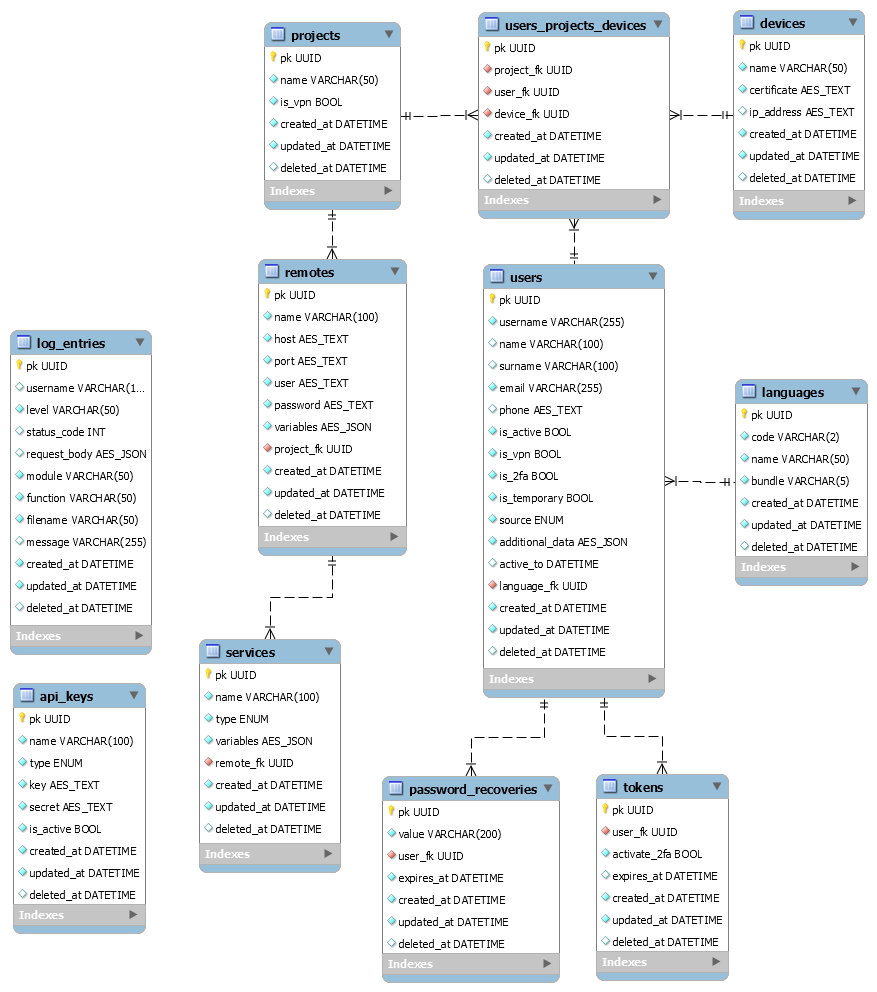
\includegraphics[width=\textwidth,height=15cm,keepaspectratio=true]{assets/eer_diagram_v2}\end{center}
\caption[Rozšírený entitno-relačný diagram]{Rozšírený entitno-relačný diagram}\label{fig:obr_13}
\end{figure}

Z databázovej schémy je možné vidieť formu uchovávania záznamov v tabuľke \inlinecode{log\_entries}, ktorá slúži na bezpečné
zaznamenávanie všetkých udalostí na strane danej webovej aplikácie.
Do tabuľky sa taktiež zaznamenávajú telá požiadaviek, ktoré používateľ v určitom čase vykonal, pričom požiadavky uchovávajúce
citlivé údaje, ako napríklad prihlasovacie údaje používateľa sa z pravidla neukladajú.
Na audtitovanie záznamov do databázy je použitá nami naimplementovaná knižnica \inlinecode{django-camel-spitter}, ktorá rozširuje
vstavaný logovací systém \inlinecode{python.logging}.

Ďalším monitorovacím rozšírením je komunikácia na službu Sentry, ktorá slúži na prehľadné zobrazovanie a sledovanie chýb v
systéme, čím pomáha pri reportovaní chýb a opravách systému.

Kryptografia zahŕňajúca, šifrovanie údajov v databáze, ukladanie hesiel a vytváranie certifikátov je obsiahnutá v knižniciach
\inlinecode{pycryptodome}, \inlinecode{pyopenssl} a \inlinecode{argon}.

Vzťah \emph{one-to-many} medzi tabuľkou \inlinecode{remotes} a \inlinecode{projects} môže byť v budúcnosti upravený na \emph{many-to-many},
pričom hodnota \emph{variables} z tabuľky \inlinecode{remotes} by sa vytiahla do separátnej tabuľky.
Ak by na určitom koncovom zariadení bolo viacero projektov, prístupy (host, port, user, password) z jednoho koncového zariadenia
by bolo možné použiť naprieč viacerými projektami, čím by sa znížila duplicita dát v databáze.
Ak sa jedná o rozdielne hodnoty (\emph{variables}) prislúchajúce koncovému zariadeniu naprieč rôznymi projektami, každý
vzťah projekt, remote a variables by bol mapovaný spájajúcou tabuľkou obsahujúcu tieto tri cudzie kľúče a utvárala by trojice.

Ak by si špecifikácia vyžadovala rozšírenie miery autorizácie riešenia, spomínanú spájajúcu tabuľku by bolo možné ďalej
rozšíriť o cudzí kľúč používateľa, prípadne aj jeho zariadenia.
Tým by bolo umožnené kontrolovať prístup používateľa nielen k danému projektu, ale aj k danému koncovému zariadeniu.

\section{SSH Poxy server}\label{sec:ssh-proxy-server}

Druhou časťou systému je samotný proxy server, ktorý je primárne postavený na knižnici \inlinecode{paramiko}.
Táto knižnica pokrýva celú implementáciu protokolu ssh verzie 2, pričom poskytuje funkcie klienta aj servera.
Proxy server musí zabezpečovať rolu ssh servera počas komunikácie s klientom a rolu klienta pri komunikácii so vzdialeným
zariadením.
Pre rozhranie servera paramiko disponuje triedou \inlinecode{ServerInterface}, ktorá je veľmi jednoducho konfigurovateľná
a rozšíriteľná.
Na druhej strane pre vytvorenie a správu spojenia cez ssh klienta je možné použiť triedu \inlinecode{SSHClient}.

Komunikáciu medzi našou webovou aplikáciou a daným proxy serverom zabezpečuje knižnica \inlinecode{praetorian-api-client},
ktorá je nami navrhnutá a implementovaná pre modulárnejšiu a jednoduchšiu správu posielaných správ.
Taktiež je týmto spôsobom umožnené všetku logiku autentifikácie a autorizácie zachovať na strane webovej aplikácie.

\section{Rozšírenie knižnice fabric}\label{sec:rozsierenie-kniznice-fabric}

Knižnica fabric je jedným z mnoha nástrojov používaných na vzdialené vykonávanie príkazov ssh, predovšetkým s cieľom konfigurácie, správy a
nasadzovania projektov pre koncové zariadenia.
Príkladom volania knižnice s cieľom nasadenia produktu môže byť nasledovný príkaz:

\begin{Verbatim}[frame=single]
fab deploy production
\end{Verbatim}

Príkaz \emph{fab}, hovorí o použití spomínanej knižnice s cieľom nájdenia súboru obsahujúceho ssh príkazy, rozdelené do funkcií podľa druhu použitia.
Druhý príkaz \emph{deploy} volá konkrétnu funkciu zo spomínaného súboru, pričom posledný príkaz \emph{production} hovorí o názve koncového zariadenia pre daný projekt.
Našou úlohou bolo túto prehľadnú funkcionalitu ponechať s cieľom rozšírenia procesu autentifikácie, autorizácie a správy citlivých údajov.

Rozšírenie s názvom \inlinecode{praetorian-fabric} pridáva do knižnice novú triedu \\ \inlinecode{PraetorianConfig}.
Konštruktor si vyžaduje iba názov projektu, pričom dodatočné informácie, ako prístupové údaje používateľa a api servera sú
získané z environment premenných.
Tým pádom sa pri vytvorení konfiguračného objektu uskutoční pripojenie na api server cez api klient s overením prístupových
údajov používateľa.
Pripojenie na ssh proxy server sa uskutočňuje až po zavolaní konkrétnej funkcie (v našom prípade \emph{deploy}), ktorá si
na vstupe žiada názov koncového zariadenia (\emph{production}).
Po zadaní údajov konfiguračný objekt typu \inlinecode{PraetorianConfig} zavolá metódu \inlinecode{connect}, kde objekt už názov
projektu a koncového zariadenia pozná.
Ak bola identita používateľa overená, je možné sa pripojiť na ssh proxy server, kde prístupové údaje
(adresa, port) sú získané taktiež z environmnent premenných.
Čo sa týka názvu používateľa a hesla ku koncovému zariadeniu, tieto údaje si uchováva databáza šifrované pomocou AES šifry.
Po úspešnom pripojení na ssh proxy server je používateľovi umožnené volať metódu \inlinecode{get\_variable}, ktorá vráti
(ako sme spomínali v štvrtej kapitole: Návrh riešenia) hodnotu citlivých údajov podľa názvu za podmienky, ak údaje môžu
byť zobrazované používateľom. Ak nie, príkaz na koncové zariadenie bude vyzerať nasledovne:

\begin{Verbatim}[frame=single]
ctx.run('mkdir {{test_file}}')
\end{Verbatim}

Pričom hodnota \emph{test\_file} reprezentuje názov dôvernej informácie, ktorej skutočnú formu vie za názov nahradiť až samotný
ssh proxy server bez možnosti používateľom zistiť jej pravú hodnotu.

Takýmto spôsobom je možné rozšíriť akýkoľvek nástroj používaný na vzdialené vykonávanie ssh príkazov, pričom neexistuje
žiadne obmedzenie medzi druhom programovacieho jazyka, frameworkom a podobne.
Z tohto dôvodu je naše riešenie viacúčelové a nepodlieha rôznorodosti technológií.
